%\documentclass[3p,twocolumn]{article}
\documentclass[12pt]{article}

\usepackage{graphicx}
\usepackage{color}
\usepackage{url}
\usepackage{ifpdf}
\usepackage{hyperref}
\usepackage{xspace}
%\usepackage[draft]{pdfdraftcopy}

\setlength\parskip{-0.015em}
\setlength\parsep{-0.15em}

\newenvironment{shortlist}{
	\vspace*{-0.85em}
  \begin{itemize}
 \setlength{\itemsep}{-0.3em}
}{
  \end{itemize}
	\vspace*{-0.6em}
}

\usepackage{fullpage}
%\usepackage[top=tlength, bottom=blength, left=llength, right=rlength]{geometry} %http://en.wikibooks.org/wiki/LaTeX/Page_Layout
%\usepackage[margin=1in, paperwidth=5.5in, paperheight=8.5in]{geometry}

\usepackage{fancyhdr}
\setlength{\headheight}{16.0pt}
\pagestyle{fancy}
\headheight = 0pt
\headsep    = 25pt
\fancyhf{}
%\fancyhead[OC]{\bf {\it \footnotesize{Jha et al: A Case for SAGA as an Access Layer for DCI}}}

\newif\ifdraft
\drafttrue
\ifdraft
 \newcommand{\amnote}[1]{  {\textcolor{magenta} {***AM: #1}}}
 \newcommand{\jhanote}[1]{ {\textcolor{red}     {***SJ: #1}}}
 \newcommand{\olenote}[1]{ {\textcolor{blue}    {***OW: #1}}}
\else
 \newcommand{\amnote}[1]{}
 \newcommand{\jhanote}[1]{}
 \newcommand{\olenote}[1]{}
\fi

\newcommand{\dn}{\vspace*{0.33em}}
\newcommand{\dnn}{\vspace*{0.66em}}
\newcommand{\dnnn}{\vspace*{1em}}
\newcommand{\uppp}{\vspace*{-1em}}
\newcommand{\upp}{\vspace*{-0.66em}}
\newcommand{\up}{\vspace*{-0.33em}}
\newcommand{\shift}{\hspace*{1.00em}}

\newcommand{\T}[1]{\texttt{#1}}
\newcommand{\I}[1]{\textit{#1}}
\newcommand{\B}[1]{\textbf{#1}}
\newcommand{\BI}[1]{\B{\I{#1}}}
\newcommand{\F}[1]{\B{[FIXME: #1]}}
\newcommand{\TODO}[1]{\textcolor{red}{\B{TODO: #1}}}

\begin{document}

\title{Characterizing Deep Sequencing Analytics using BFAST: Towards a
  Scalable Distributed Architecture for Next Generation Gene
  Sequencing}

\author{Joohyun Kim$^{1}$, Sharath Maddineni$^{1}$, Shantenu Jha$^{*1,2}$, \\
  \small{\emph{$^{1}$Center for Computation \& Technology, Louisiana State University, USA}}\\
  \small{\emph{$^{2}$Department of Computer Science, Louisiana State University, USA}}\\
  \small{\emph{$^{*}$Contact Author \texttt{sjha@cct.lsu.edu}}}
  }


\maketitle

\section*{Abstract}

Next-Generation (gene) Sequencing (NGS) machines produce significantly larger amounts of data compared to early sequencers.  In addition to the challenge of data-management that arise from unprecedented volumes of data, there exist the important requirement of effectively analyzing the data.  In this paper, we use BFAST -- genome-wide mapping application, as a representative example of the typical analysis that is required on data from NGS machines.  

We investigate two model genomes -- human genome and a microbe, Burkerholderia Glumae, that represent an eukaryotic and a prokaryotic system.  The computational complexity % of execution of bioinformatics calculation,
of mapping with BFAST, depends upon the size of a reference genome, the data size of short reads from high-throughput technologies of the Next Generation Sequencing platforms, and their biological genome contexts such as distinctive differences between prokaryotes vs eukaryotes.
We analyze the performance characteristics of BFAST, understand its dependency on different input parameters and for typical data-volumes. 

We then investigate the use of distributed computing environments, a production HPC grid and a cloud environment for the genome-wide mapping with BFAST.  The two distributed environments, the Louisiana Optical Network Initiative (LONI) grid and a Cloud system from the FutureGrid, were used primarily focusing on different and unique challenges in HPC and Cloud computing conditions.

% The main goal of this work is to understand the
% characteristics of these two distributed computing environments and
% compare and contrast their strengths and suitability to support the
% computational requirements of deep sequencing.

% regarding computational requirements of the target bioinformatics application whose

\jhanote{This needs to be refined/modified} The time to completion is analyzed by comparing advantages as well as limitations of each distributed computing infrastructure in conjunction with distinctively different two different genome systems.  With our results, we discuss the importance of an effective runtime environment that facilitates a rapid development of cyberinfrastructure of distributed computing resources and supports optimized execution patterns for a target scientific application, in particular, of the data-intensive genome-wide analysis.


\section{Introduction}

% \bibliographystyle{plain}
% \bibliography{egi-white-paper}
High-throughput sequencing techniques provided by Next Generation Sequencing (NGS) platforms have changed biological
sciences and biomedical research dramatically with their comprehensive genome-wide
information as well as a considerably affordable cost compared to previous sequencing techniques based on Sanger sequencing\cite{metzker2010,mardis2008-tig,mardis2008-arghg,gilad2009,mortazavi2008,sorek2010}.  
Owing to the advances in deep sequencing protocols such as ChIP-seq and RNA-seq, high-throughput sequencing techniques becomes essential methodologies in studies of cell development and differentiation\cite{wang2009-natrevgen,pepke2009,gilad2009,mortazavi2008,sorek2010}.   Resulting influx of biological information about the genome-wide organization and the interaction map of target genes or pathways that reveal underlying mechanisms of gene expression and regulation in a living cell would lead to discoveries of remedies for various diseases such as cancer, infectious diseases, and dysfunctional diseases caused genetically or by aging\cite{amaral2008,encode2007,baek2008,costa2009,}.    

While high-throughput techniques enjoy extremely high coverage of target genome regions, as referred often with the term, "deep sequencing", the current technologies adopted by NGS platforms such as Illumina GA II and Applied Biosystems SOLiD are limited to generate only short sequence reads generally less than 100 hundred nucleotides in a real setting at the time of this writing\cite{metzker2010}.  Consequently, these high volume short reads challenge immediately mapping process on to a reference genome or de novo assembly that are  needed as the first step for any genome-wide studies\cite{alex2009,trapnell2009,scheibye-alsing2009,pop2002,hernandez2008,farrer2008}.      

The need of computational methods as well as computing architectures for compute-intensive and data-intensive calculations for resolving new challenges arising from requirements of processing and analyzing genome sequencing data, therefore, is regarded indispensable for accurate and reliable analysis against high-throughput sequencing data and following genome-wide analyses.  As a result, remarkable advances have been witnessed in recent years and a number of bioinformatics tools aiming to solve emerging challenges are currently available to the scientific community\cite{trapnell2009,bfast2009,scheibye-alsing2009,pepke2009,samtools}.  One important caveat is that as advances of genome sequencing technologies evolve further in the future with innovations, for example, such as a single molecule sequencing technology and ever-growing genome data, any computational algorithms or implementations with a bioinformatic tool are subject to change to respond such progresses or will become less useful if the tool do not meet new conditions. 

Whereas such algorithmic advances and introduction of new tools have been consistently led by the computational biology community. the development of infrastructure and required software is relatively less recognized for its significance.  This is partly because, in addition to requirement of an understanding of applications of interest in terms of the capability of parallel execution in heterogeneous computing environment, the complexity of biological contexts associated with characteristics of a target genome(s), the volume of relevant genomics data, and importantly, difficulties of utilization of heterogeneous distributed computing resources constitute challenges for introducing an appropriate scalable architecture for the infrastructure.

Nonetheless, some interesting progresses are recently reported, for example, with the utilization of emerging computing architecture such as Cloud\cite{taylor2010}  In this work, we report our development on the distributed adaptive runtime environment (DARE) framework with which heterogeneous distributed computing resources are keenly utilized for a scalable computation of a target genome-wide analysis tool.  As a use case, we primarily focus on the mapping process of short reads from NGS platforms against a reference genome.  The mapping is carried out with the tool, BFAST\cite{bfast2009, bfast2009b} which was chosen specifically considering its capability to support parallel and multi-threading execution.  Our investigation with this bioinformatic program would represent a general situation for a bioinformatics tool employed for genome-wide analysis infrastructure.

\jhanote{we want to present a strawman of an architecture based upon
  requirements and a reference implementation of the architecture} In
this work, we present our work on the infrastructure development for
the use of High Performance Computing (HPC) grids and Cloud
environment for genome-wide analysis.

Our strategy is, first to understand characteristics of biological information in conjunction with the capability of the target scientific application, and then, to analyze computational complexity for carrying out mapping process with two exemplary genomes, human genome and a microbial genome, Bukerholderia Glumae.  Base on the results with this analysis, we present the use of the runtime environment developed with the Distributed Adaptive Runtime Environment (DARE) framework, which is built upon SAGA/BigJob abstraction and provides an efficient framework for building biological information infrastructure supporting a wide range of execution patterns while recognizing the potential scalability of deployable computing resources.  Our development with a federated HPC grid, Louisiana Optical Network Initiative (LONI) and a Cloud environment in the FutureGrid is desribed largely focusing on the comparative analysis on execution of mapping process in each environment. 


%First, we note that in general, genome-wide mapping procedure is an good example of data-intensive scientific applications and can be efficiently carried out with parallel or concurrent executions if there exist ways of data fragmentation with intact biological information.  For example, a reference genome is likely to be composed of many chromosomes or plasmids, and thus mapping on each chromosomes and plasmids can be executed separately.  The challenge, however, is that the way of data fragmentation, and thus system configuration for required parallel/concurrent runs should be considered the characteristics of system environment. Those characteristics differ distinctively between a HPC grid and a Cloud and also vary with a specific target system in each class.  


\section{Mapping with BFAST with Two Genome Datasets: Scientific and Computing Challenges}

\subsection{BFAST : Application}

Our target genome analysis tool is a mapping tool, BFAST\cite{bfast2009,bfast2009b}, which represents a class of tools that comprises diverse genome-wide analysis applications but shares similar computational features.  Such features include i) a requirement of input files containing sequence information of a reference genome or short reads from NGS platforms ii) a production of output files that is generally written with a format that is successively injected to another tool as input.  These aspects, along with a huge variation in the data volume in input, output, or temporary files, often require that the tool should support parallel or multi-threading executions, which is also true with BFAST\cite{bfast2009}.

As summarized in Fig.~\ref{fig:workflow-bfast} and Table~\ref{table:bfast-summary}, BFAST carries out a pipeline that comprises six different steps (using a different command), and compute extensive steps could be executed in parallel or multi-threading support options.  In brief, BFAST requires a reference genome sequence and NGS platform generated short reads initially and prepare input files with pre-defined formats.  Then, the program carries out indexing of the reference genome, finding Candidate Alignment Locations (CALs), local alignment of CALs, and post-processing of alignment results, which taken together produces the mapping of billions of short reads onto the target reference genome.  Among the steps, three steps (index, match, loalalign) demands most of computing times and computing requirements with the size of a reference genome as well as volumes of short reads.  If computing requirement is high, as stated, BFAST can be executed using parallel or concurrent options by splitting the input data, short reads and a reference genome and run many independent tasks with a part of datasets.  For example, short reads files can be prepared with multiple files and short reads in each file are mapped independently against a reference genome.  Meanwhile, where as a reference genome is also split into many files by considering the existence of multiple contigs in an entire genome, for example, multiple chromosomes and plasmids, in the case of one large sequence, all information about indexing should be treated as a whole for "match" step. 

BFAST also supports multi-threading and the low memory option for "match" step. Once a reference genome sequence is given and not able to be split into further, creating indexes of the reference genome with multiple index files are possible resulting the number of the index files, $N_i$ equal to $n_m \times 4^d$ where d is the parameter for the low memory consumption and $4^d$ files are generated by splitting an index file.  $n_m$ is the number of masks for indexing and usually fixed as 10 for our work.  Whereas this low memory option allows to consume less memory by splitting the information about index into many files and processing sequentially, the number of index files increases.  Another important option provided by BFAST is multi-threading.  If there is multi-core in a node, the option can specify the number of cores for multi-threading.    

\begin{figure}
 \centering
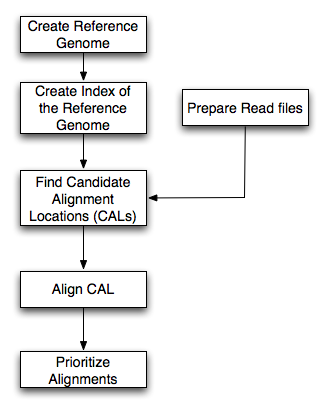
\includegraphics[scale=0.45]{figures/workflow.png} 

\caption{\small Overall workflow for a mapping procedure using BFAST.  In this work, we focus on the step for finding Candidate Alignment Locations (CALs).  }
  \label{fig:workflow-bfast} 
 \end{figure}


\begin{table}
\begin{tabular}{|c|c|c|c|} 
  \hline 
 BFAST command & Description & Supported \\ 
  &  &     Parallelism \\\hline
\texttt{bfast fasta2brg} & creation of a ref. genome  &    multiple independent contigs \\
&  preparation of short reads files &     multiple sequence reads files \\

\texttt{bfast index} & creation of reference genome indexes& multi-threading, split index file creation\\
\texttt{bfast match} & finding candidate alignment locations  &  multi-threading, parallel execution \\
\texttt{bfast localalign} & alignment of each CAL  &   parallel execution \\
\texttt{bfast postprocess} & prioritization of alignments  &  parallel execution \\ \hline


\hline
\end{tabular} \caption{Description of BFAST commands and features that can be used for parallel/concurrent and multi-threading execution}
 \label{table:bfast-summary} 
\end{table}

%Note that the number of required
%concurrent tasks, $N$, 


\subsection{BFAST: Characteristics}

\begin{figure}
 \centering
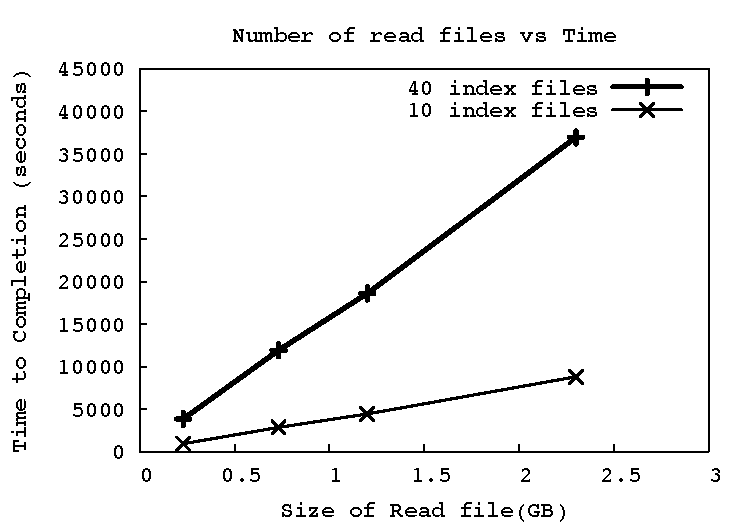
\includegraphics[scale=0.66]{figures/readsvstime.pdf}
%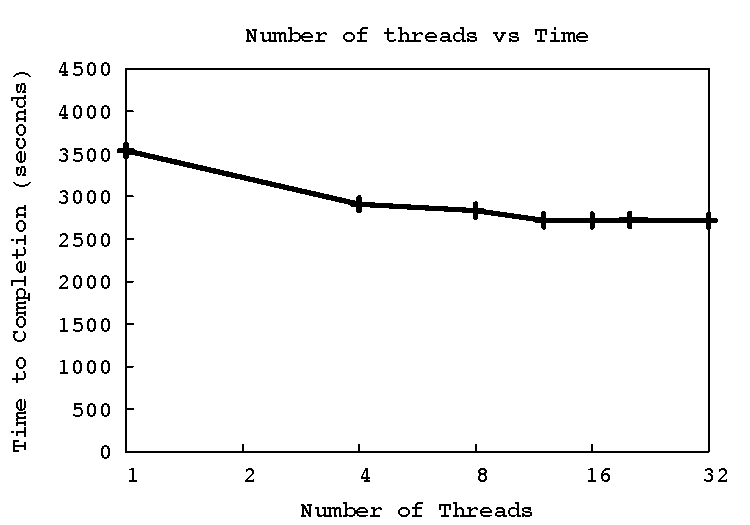
\includegraphics[scale=0.66]{figures/threadsvstime.pdf} 

\caption{\small Parallel execution support in BFAST.  ``Match''step is measured by changing the size of short reads file and low memory option (left) and multi-threading support (right).  Human genome (hg18) chromosome 21 is used as the reference genome. \jhanote{Need to say what the two lines in the left graph are, and what is the message we want to convey from showing the difference} \jhanote{I think we should use gnuplot for production quality graphs. Sorry -- but the quality makes a significant difference and Excel just does not cut it.}}
  \label{fig:parallel-execution} 
 \end{figure}


The time-to-solution for "match" step depends upon several parameters that determine the configuration for parallel tasks and multi-threading support.  Computational resource specification such as the size of memory, accessible volume of disk space, the number of cores in a node, and the total number of cores available are the important information for optimal condition for such parameters.  An understanding of such aspects was attempted by characterizing computing characteristics of the "bfast match" step.  The results from our investigation are presented  in Fig.~\ref{fig:parallel-execution}. First, performance gains with multi-threading are marginal showing only 30 \% speed up when reaches the limit with all of the number of free cores being used.  
Secondly, the multiple reads file option is useful as a strategy for scaling out, i.e. with more cores operating correspondingly a smaller reads file.  Thirdly, the low memory option that creates more index files require longer calculation time as the comparison between 40 index files $(d = 1)$ vs. 10 index files ($ d = 0 $) and $n_m = 10$.   





\begin{table}
\begin{tabular}{|ccc|} 
  \hline 
   & Human (hg18) & Burkerholderia Glumae (BGR1)  \\ \hline
 \underline{\textbf{Reference Genome}}   \\
    \# of base pairs (bp) &  3 Gbp & 7.3 Mbp \\
   Genome Structure &   23 chromosome pairs  & 2 chromosomes \& 4 plasmids  \\  
    Volume of indexes  & approx. 12 GB  & approx. 447 MB  \\
    \underline{ \textbf{Short Reads Sequence Data}}   \\
  Type of Genome Analysis &  Exome  & Whole Genome Resequencing \\
  Sequencing Platform & ABI SOLiD  &  Illumina GA2 \\
  Sequencing Data Volume  & 8.7 GB & 5.4 GB \\
  \underline{ \textbf{BFAST mapping} }  \\
  Minimal disk space required  &  approx. 130 GB   &    approx. 10 GB   \\

\hline
\end{tabular} \caption{The information about the size of reference genomes, volumes of datasets from Next Generation Sequencing (NGS) platforms and disk space required during the mapping calculation with BFAST is summarized assuming all calculations are carried out with a single machine.}
 \label{table:two-genomes} 
\end{table}

\subsubsection{Computational Requirements}

Computational requirements for carrying out BFAST steps, in particular the "bfast match" step are associated with biological contexts such as a type of a target reference genome and high-throughput sequencing techniques generating short reads sequences, parallel/multi-threading execution pattern, and available computing architectures.  

The difference of computational requirements arising from different genomes could be hinted with two genome datasets that are representative of biological diversity, an eucaryote system, human, and a microbe, Burkerholderia Glumae\cite{kim2011}.  Two genomes differ in the size and the genome structure of reference genomes, types of sequencing protocols for generating short reads and consequently different mapping rates, which is summarized in Table~\ref{table:two-genomes}.  Importantly, the two different genomes display widely different data sizes in terms of the reference genome sequence, short reads data, and required disk space for carrying out the mapping with BFAST as presented in Table~\ref{table:two-genomes}. 

Computational requirements vary also with how to configure parallel/multi-threading execution patterns.  Since BFAST provides its intrinsic support for multi-threading and parallel execution, we examined computational requirements while varying configurations for such parallel strategies.  For example, according to the results shown in Fig.~\ref{fig:parallel-execution}, it is obvious that dividing a large volume of short reads data into many independent runs is a good strategy while multi-threading support is limited by available cores in a same node.  Also the results in Fig.~\ref{fig:parallel-execution} find that the low memory option that allows to split one index file into many do not benefit in the computing time. Our results suggest that the size of an index file affects on the total time to solution marginally while the size of a short read file is the determinant factor, indicating that the low memory option needs an increase of the computing time as the number of calculations with a short read file becomes as multiple as the number of divided index files.   

Most importantly, while the implementation of multiple parallel tasks indicates advantages of distributed multiple resource utilization, the large volume and variation of data sizes associated with genome sequence data as well as minimally required disk space needs to pay attention since in some cases, data size itself prohibits to carry out the analysis in a computing resource that lacks the demanded requirements, indicating the significance of agile runtime environment that drives a dynamical configuration and utilization of distributed resources. 




\jhanote{Joohyun: Please organize each description addressing each of
  the following points: (i) Brief outline of the scientific problem,
  (ii) What are the challenges, (iii) estimates of volumes of data
  involved, distributed or not?, number of tasks, are they coupled or
  uncoupled -- what is the level of coupling between tasks?}


 \begin{table}
 \begin{tabular}{|c|cc|} 
 \hline 
Distributed Environment &  HPC Grid &  Cloud \\ \hline
System  &  Louisiana Optical Network Initiative & FutureGrid \\
Name &  QB/Eric   &  INDIA/SIERRA \\
 \hline
 \end{tabular}
\caption{Specification of two distributed environments}
\label{table:two-systems} 
\end{table}
 
\subsubsection{BFAST: Characterising Data Requirements}

\jhanote{Lines 86-87, In a nutshell: the operating data-set does not depend on the size/number of read files but does depend on the size/number of index files}

Another interesting observation is, as shown in Fig.~\ref{diskspace}, that the requirement for disk space is lessened as more distributing resources are utilized. The reason is that multiple concurrent tasks corresponding to multiple reads files require more disk space due to temporary files for each task, and distributed data storage is beneficial, in particular, for an architecture that does not provide a large disk space.  For example, the Cloud system we examine here do not provide a large volume, and even in the LONI grid, small cluster machines are hard to support an individual account more that 100 GB.

\begin{figure}
 \centering
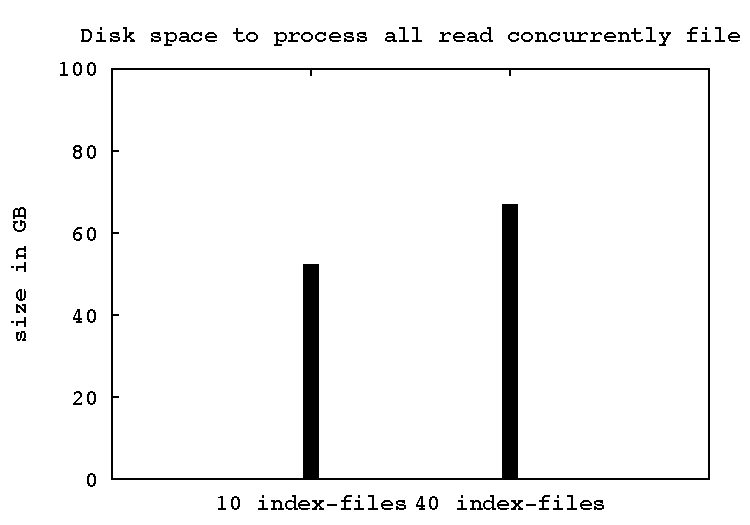
\includegraphics[scale=0.66]{figures/diskspace.pdf}
\caption{\small Disk space requirement in the case that all reads
  files are processed concurrently in a single storage is compared to
  the case when each single reads file is processed with a distributed
  storage.  Also, the comparison of the required disk space for the
  low memory option that produce 40 index files with the normal
  configuration that produce 10 index files is presented. \jhanote{We
    need to increase the font of the labels in the figure. Almost
    impossible to read. Should be easy in gnuplot..} \jhanote{Remove C and D ot later possibly}}
  \label{fig:diskspace} 
 \end{figure}

\section{Mapping with BFAST Using Distributed, Scalable Architectures}

\subsection{Existing Solutions: Limitations and Challenges}

\jhanote{Here we need to define what solutions are currently employed, what works well
  what doesn't}

Recently, cloud computing and environments for genome-wide analysis and infrastructure development have drawn significant attention and interesting outcomes were reported\cite{taylor2010,cloudburst, cloudblast, langmead2009, langmead2010,gatk, halligan2009}

\begin{itemize}
\item GATK\cite{gatk}
\item CloudBurst\cite{cloudburst}
\item CouldBlast\cite{cloudblast}
\item SNP finding and RNA-seq with Cloud\cite{langmead2009, langmead2010}
\end{itemize}

In spite of successful progresses from such efforts, the primary challenges that we want to resolve, and improve are as follow.

\begin{enumerate}
\item Agility for heterogeneous computing architecture
\item Extensibility and quick development cycles for a new bioinformatics tool
\item Scalability with a non-intrusive execution of a target tool  
\end{enumerate}

\subsection{Distributed Adaptive Runtime Environment}

To execute a scientific application using heterogeneous distributed computing resources, we develop the Distributed Adaptive Runtime Environment (DARE) framework\cite{dareurl}.  The framework is compose of an open source Web application framework, Pylons
and middleware of the application management system built upon SAGA an BigJob abstraction\cite{saga-ccgrid10,saga-royalsoc,saga-web,jha2009developing,ecmls10}.  This combination of the open source technology and the application management system enables us to develop a lightweight, extensible, full-fledged distributed computing science gateway quickly and effectively\cite{pylonsurl}. 

Considering a daunting size of data, in particular large genomes such as human as summarized in Table~\ref{table:two-genomes} and corresponding long computing times when carried out with a single or moderate size of clusters, parallel/concurrent execution of the target analysis with BFAST are desirable.  First, biological information could be utilized for such parallel execution. For example, the short reads sequences in fastq format could be split into many files that are needed separately for parallel mapping.  At the last stage, all mapped results could be combined with available tools such as SAMTools\cite{samtools}.   Additionally, a reference genome could be divided into many if each dataset contains independent contigs.  For example, each chromosomes or plasmids in microbes could be a separated sub-genome sequence contig.  However, note that indexes of an entire contig should be used together, regardless of the low memory option that allows to store indexes in many files, which is in fact the major obstacle to require a large disk space.

We implement the above data fragmentation scheme on grids and clouds with the same runtime environment using SAGA/BigJob\cite{saga-royalsoc,saga-ccgrid10, ecmls10}.  In our implementation, all the parallel tasks of BFAST steps are defined as SubJobs in BigJobs.  It is possible to assign many cores for each SubJob with the configuration of BigJob before submitting BigJobs. 
  
In the Grid implementation first all the data required in the steps was transferred to machine's  work 
directory where we want to start the BigJob. The BFAST was installed in the home directory and the
executables path for job description of subjobs was given accordingly.

In the cloud implementation all the data required was transferred into the walrus because of the data size limitation of the storage space in the
running VM. Multiple VM's can be started at once and the data in the walrus is mounted onto all the running VM
while booting the Virtual Machine. Thus all the VM can have access to data and can process concurrently


\subsection{Understanding BFAST Dependence on a Local Resource}

\subsubsection{$T_{C}$ on $N_t$ and $N_c$}

 \begin{figure}
 \centering
%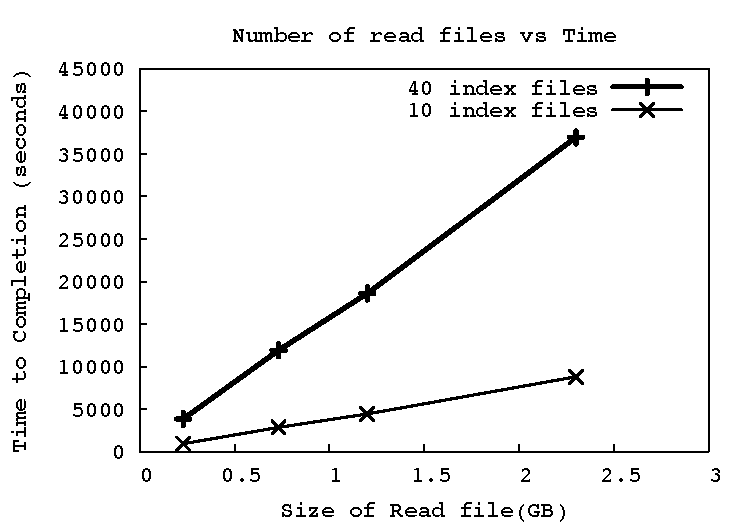
\includegraphics[scale=0.66]{figures/readsvstime.pdf}
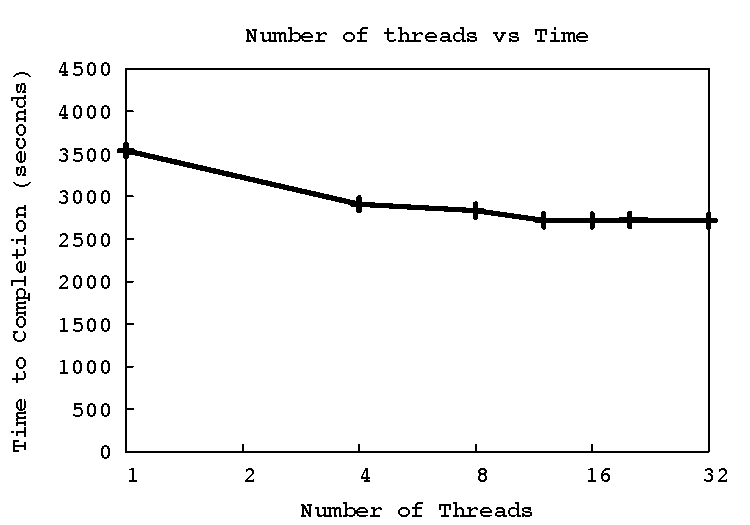
\includegraphics[scale=0.66]{figures/threadsvstime.pdf} 

\caption{\small Parallel execution support in BFAST.  ``Match''step is measured by changing the size of short reads file and low memory option (left) and multi-threading support (right).  Human genome (hg18) chromosome 21 is used as the reference genome. \jhanote{Need to say what the two lines in the left graph are, and what is the message we want to convey from showing the difference} \jhanote{I think we should use gnuplot for production quality graphs. Sorry -- but the quality makes a significant difference and Excel just does not cut it.}}
  \label{fig:parallel-execution} 
 \end{figure}


\subsubsection{Understanding I/O}
{
To understand the how I/O of the system influences the performance of bfast matching four different experiments were conducted keeping the amount of data processed constant and number of threads used also as constant but for the first three. In the first experiment we just perform one bfast match for a large reads file of size with four threads and four cores. In the second experiment two bfast matches concurrently with almost half the size of reads file but half of the threads used in the first one.Similarly, in the third experiment we run four bfast matches concurrently with almost quarter the size reads file used but the in the first experiment and one thread each. Fourth one is similar to third except in the number of threads 4 threads per bfast job is used but using just 4 cores.

 \begin{table}
 \begin{tabular}{|c|c|c|} 
 \hline 
Reads file size in GB &  Number of threads per Reads file & Time to completion in seconds \\ \hline
2.3 &  4 & 36942  \\
1.2 & 2 & 19618 \\
0.732 & 1 & 28299\\ 
0.732 & 1 & 25215\\

 \hline
 \end{tabular}
 \label{table:understand I/o} 
\end{table}


These experiments show that use of 2 threads per bfast matches simultaneously on a four core node is the optimal configuration for time to completion. Because it balances each thread per core but  running the two bfast jobs per node at the same time. Thus shows advantage of running multiple bfast matches simultaneously. 


}

\jhanote{Lines 44-47 of the Excel Sheet here}

\subsection{Experiments with HPC and Cloud}

\subsubsection{Using BFAST On Distributed Grids}

Following is the implementation described above, the execution of mapping calculations using BFAST was tested with our runtime environment built with the DARE framework.   Results were obtained with a HPC grid and a Cloud environment, which demonstrate the capability of our runtime environment for the mapping tool on distributed heterogeneous computing resources. \jhanote{Before we say what we are presenting, please present a ``why and how'', i.e., outline the experiments} 

First of all, in Table~\ref{table:bigjob-loni}, we presented the measured time-to-solution for the step 'bfast match' with different configurations that include the variation of the number of threading used for each task and the number of cores (and also the number of nodes).   These results clearly show i) effective job submission and sub task management trough BigJob in spite of a large number of subtasks up to 40 ii) requirement of sufficient number of cores through available distributed computing resources (see I and II compared to III and IV that requires many rounds of parallel executions due to limited number of cores) that completes parallelism with multiple reads files.  In particularly, the observation with (ii), along with the observation already shown in Fig.~\ref{fig:parallel-execution} that observed a marginal performance gain with the option for increasing number of threading, is clearly supported by the results shown in Fig.~\ref{} once again that shows the result in that without sufficient cores available from distributed resources and dynamically adapted task distribution, achieving the efficient execution of a target calculation is challenging.


 \begin{table}
 \begin{tabular}{|ccccc|c |} 
 \hline 
ID & BigJob Size  &  \# of Tasks & Size of  & \# of Thread  &   Computing  \\
   & \# of Cores (\# of Nodes) &  & Reads File & for Each Task &  Time\\\hline
I   & 80  (8) &  40 & 0.209 GB & 2 & 1h 6 m 6 s \\
II  & 40 (8)  &  20 & 0.435 GB & 2 & 2 h 13 m 51 s\\
III & 12 (4)  & 40  & 0.209 GB & 2 & 7 h 10 m 7 s \\
IV & 12 (4)  & 20 & 0.435 GB & 2 &  6 h 37 m 52  \\
\hline
\end{tabular}
\caption{Performance comparison among parallel implementation using SAGA/BigJob with a HPC grid, LONI. One BigJob is submitted with the number of SubJobs indicated in the column for the number of tasks which is equivalent to the number of reads files.\jhanote{The result -- IIUC, is the second column. This should come last and separated from the other columns 3- 6 are used to understand the configuration, and so should be with the first column}}
  \label{table:bigjob-loni} 
\end{table}
 


\subsubsection{Using BFAST on Clouds and Grids}


\section{Concluding Remarks}
We present our analyses with two genome systems representing a eukaryote and a prokaryote, respectively, using
 a HPC grid and a Cloud environment for an understanding of conditions of a scalable cyberinfrastructure for an effective execution of
 mapping, and consequently genome-wide analyses.   Based on our results, we conclude that an infrastructure to run with a proper configuration for concurrent tasks benefits genome-wide analysis and such a configuration is optimized only when parameters from biological contexts as well as limitations and potentials of distributed computational resources are taken into account together.  For that purpose, our DARE framework provides an efficient solution.  



\bibliographystyle{abbrv}
\bibliography{ecmls11}


\end{document}

